\chapter{Estado de la cuestión}
\label{chap:estado_cuestion}

En la actualidad, la generación de música o, en un sentido ámplio, de sonido, constituye uno de los frentes de investigación activos y más prometedores en el campo de la IA. La generación música con modelos de \textit{Deep Learning} ha sido abordado históricamente desde dos grandes perspectivas en función de la naturaleza de los datos generados por los modelos: la generación de música simbólica y la generación de música con audio. La primera de ellas consiste en la creación de elementos musicales como notas, acordes, melodías, etc. en un formato simbólico, ya sea MIDI, OSC, MusicXML, ABC, Lilypond, o cualquier formato musical reducible a símbolos textuales. La segunda, en la creación de un flujo de audio directamente reproducible sin necesidad de síntesis sonora o utilización de bibliotecas de \textit{samples}.

La primera aproximación, la de la composición informática de música a través de elementos simbólicos, se remonta a los inicios de la computación, con pioneros como Lejaren Hiller y Leonard Isaacson, que en 1957 crearon \textit{Illiac Suite} \cite{arizaTwoPioneeringProjects2011}, la primera composición musical generada por ordenador. Desde entonces, la generación de música simbólica ha sido abordada desde diferentes perspectivas, como la generación de música aleatoria, la generación de música a partir de reglas, la generación de música a partir de modelos probabilísticos como las cadenas de Markov, música basada en mátemática fractal, estocástica, etc. \cite{hernandez-olivanSurveyArtificialIntelligence2022}. 


La generación de audio por medio de modelos de \textit{Deep Learning} es un campo de investigación más reciente debido en parte a su gran demanda computacional, que ha estado fuera del alcance de investigadores y empresas hasta la última década. Actualmente, modelos como \textit{MuseNet}  \cite{departmentofcomputersciencesrminstituteofscienceandtechnologychennaiindia.MusenetMusicGeneration2020a}, \textit{Jukebox} \cite{dhariwalJukeboxGenerativeModel2020}, \textit{Stable Audio} \cite{StableAudioFast}, o \textit{Suno} \cite{SunoAI}, entre otros, han sido capaces de generar música con audio de una alta calidad, y, al igual que está ocurriendo con modelos de generación de imagen o vídeo, se espera que en los próximos años se produzcan avances muy significativos en este campo.

En este trabajo, el foco está puesto en la generación de música simbólica, y más concretamente, en la generación de código de programación sonora. Esta aproximación hubiera sido impensable antes de la aparición de los grandes modelos de lenguaje, los cuales se basan en la arquitectura \textit{Transformer}, aparecida en 2017 \cite{vaswaniAttentionAllYou2017}, por lo que es un tema de investigación muy reciente. Por otra parte, todas la investigaciones candentes en este momento se están centrando en la generación de audio, campo más prometedor desde el punto de vista comercial. 

La generación de código de programación por LLM, independientemente de su finalidad artística o técnica, sí que es un campo estudiado en los últimos meses, y que ha dado lugar a la aparición de modelos como \textit{Github Copilot}, que ha sido capaz de generar código de programación de considerable calidad a partir de inputs o \textit{prompts} en lenguaje natural.
 


\begin{itemize}
    \item Modelos de IA generativa aplicados a la música.
    \item LLM asistentes para la creación de código de programación.
    \item Lenguajes de programación musical.
    \item Prompting engineering.
    \item LLM y música (MIDI y otras representaciones).
    \item LLM y música con lenguajes de programación.
\end{itemize}

\section{Modelos de IA generativa aplicados a la música}
    Repasar especialmente los últimos modelos lanzados por Google y Amazon\dots y su estado.

\section{LLM asistentes para la creación de código de programación}
\label{sec:llm_asistentes_creacion_codigo_programacion}
    GPT-4 como estado del arte. Software específico como Github Copilot. Hablar de los más importantes LLM y su rendimiento en la programación.


    \begin{figure}[h]
        \caption{Habilidades de los \textit{Foundation Models} de OpenAI.}
        \centering
        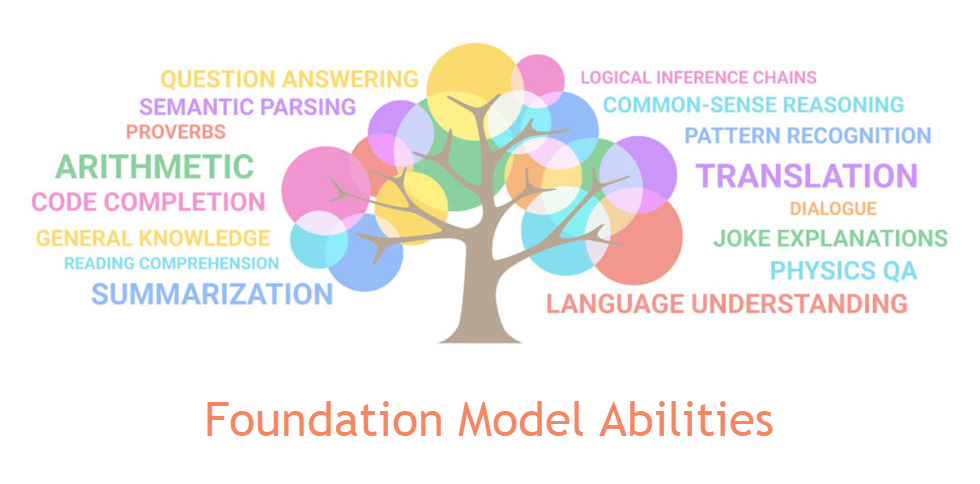
\includegraphics[width=0.8\textwidth]{./figuras/fundation_models_habilities.png}
        \source{\cite{GPT3RiseFoundation}}
        \label{fig:fundation_models_habilities}
    \end{figure}

\section{Lenguajes de programación musical}
    Lenguajes a modo de código de programación, como Overtone, Pure Data, Sonic Pi, Supercollider, Max MSP. Representaciones musicales susceptibles de ser generadas por LLM, como el MIDI, MusicXML, ABC, Lilypond, etc.

\section{Prompting engineering. Estado del arte}
    Un repaso por los papers más significativos y actuales sobre esta cuestión, especialmente las que implican la generación de código.

\section{\textit{Retrieval-Augmented Generation} (RAG)}
    Una de las técnicas más potentes para la generación de código, que combina la recuperación de información con la generación de texto. También de OpenAI Assistant, que ha presentado en el Keynote de 2023. \cite{WhatRetrievalaugmentedGeneration2021} y \cite{lewisRetrievalAugmentedGenerationKnowledgeIntensive2021}

\section{LLM y música (MIDI y otras representaciones) y el problema del significado}
    Quiero exponer la distancia que supone conocer un lenguaje y usarlo para crear arte con él. Que un sistema (o un ser humano) conozca la sintaxis de un lenguaje no significa que pueda crear con él obras de arte... al menos si no se le entrena con suficientes datos.
    
    Usar como bibliografía: el paper \cite{lewisRetrievalAugmentedGenerationKnowledgeIntensive2021} y la web \cite{WhatRetrievalaugmentedGeneration2021}

\section{LLM y música en SuperCollider}